

\chapter{Hardness of Application of Rewrite Rules} \label{sec:hardnessrewriterules}
Now that we have explained the background for string rewrite systems, as well as the motivation for them, we now build on top of the  algebraic hardness measure computation done in chapter~\ref{sec:subhrdnspred}. First, we discuss a program we created that replays the Collatz SRS for certain numbers, which is used throughout this chapter. Then, we attempt to establish a reasonable upper bound for number of rewrite steps needed. We then use this upper bound to compute reasonable hardness measures for modifications of the Collatz SRS that align with the earlier discussed variants. Finally, we explore another modification to Aaronson's rewrite system which reduces rewrite steps.% First, we do computations with slight modifications to the Collatz SRS, and second, we only compute record sequences from our previous algebraic analysis. In this section, we first introduce a modified version of the SRS, then we define measures, talk about the computation, then present our results.
\section{Computation} \label{subsec:rewritecomp}
The program we wrote simulates the Collatz SRS in Java. It takes two different required inputs: some positive integers (either one number, or a batch of numbers, one per line), and a string file which has one SRR per line in the format ``input output'', which is equivalent to the rule $input \rightarrow output$. The \# character is a comment, meaning if the first character of a rewrite rule is \#, we ignore that line. This is a convenience to comment out a rule to create SRRs that correspond to Collatz subproblems. The output is a file with the transformation of the rewrite terms, and which number these terms correspond to. If a batch of numbers is run, one file is made for each number. Also, an aggregate file can be printed for batches that lists, for each input number, a row that has the input number, the final number, and the number of rewrite steps. \par
The program converts an input number into a binary rewrite string with characters $a$, $b$, $c$, and $d$. The rewrite term is stored in an array that has a ``sliding'' string in it. This is the most efficient way to take advantage of Aaronson's SRS, because a number only grows from the $c$ term, and shrinks from the $d$ term. Hence, the spare space of the array is past the $c$ term, and any time a $D$ rule decreases size, we move in the end of the $d$ symbol, and all other symbols past it are thrown out if more space is needed. For instance, when we apply rule $D_2$, the $a$ term gets replaced with a $d$ term, and a pointer denoting the end of the string gets moved to the new $d$ symbol. If we run out of space in the array, we double the size of it, discarding any unnecessary terms past the $d$ symbol with a pointer. \par
As discussed in section~\ref{subsec:CollatzSRS}, we don't apply SRRs in arbitrary order. Given a rewrite string completely in binary, we check to see if any $D$ rule can be applied. If not, the program terminates. If we do find a $D$ rule, then apply it, and check if a ternary character is generated by it. If so, we apply the $A$ and $B$ rules to move the ternary character index-by-index until we can apply a $C$ rule, which removes the ternary character. \par
The code can be accessed via a public GitHub repository located at \url{https://github.com/mdenend/CollatzRewriteSystem}. A readme file is included that explains how to run the code and available options.


\section{Estimated rewrite steps needed} \label{subsec:estrwsteps}
Looking at how the Collatz SRS operates, one can establish a reasonable bound on how many more steps the Collatz SRS adds compared to the algebraic method of computing Collatz Sequences. Starting with a number that is purely in binary symbols $a$ and $b$, plus the placeholder symbols $c$ and $d$, there are two different events that can occur. When $a$ is the symbol to the immediate left of the $d$, we divide by 2. It only takes one step to complete this division. On the other hand, when a $b$ symbols is to the immediate left of the $d$, we turn the $b$ symbol into a $g$ symbol to effectively compute $(3x+1)/2$, and, following the establised order, apply $A$, $B$, and $C$ rules to convert the ternary symbol to binary. This adds $\Theta(m)$ rewrite steps per odd number. \par
We can compare the number of steps that the rewrite system takes to Classical Hardness records from chapter~\ref{sec:subhrdnspred}. Let $m$ in this case be the bits for Classical Hardness record $r$. If we do in fact apply a factor of $\Theta(m)$ more steps per odd number in our rewrite system, then Classical Hardness should be pretty close to $\text{``Rewrite Steps Added by Odd Numbers''}/\log^2{r}$ for Classical Hardness records input into the Collatz SRS. The results of this analysis are presented in Figure~\ref{fig:rvc_log}. From this graph, it appears that dividing the odd number of rewrite steps by $\log^2{r}$ creates a reasonably tight bound against Classical Hardness, so the Collatz SRS adding a factor of $\Theta(m)$ rewrite steps per odd number appears to be correct.
\begin{figure}
    \centering
    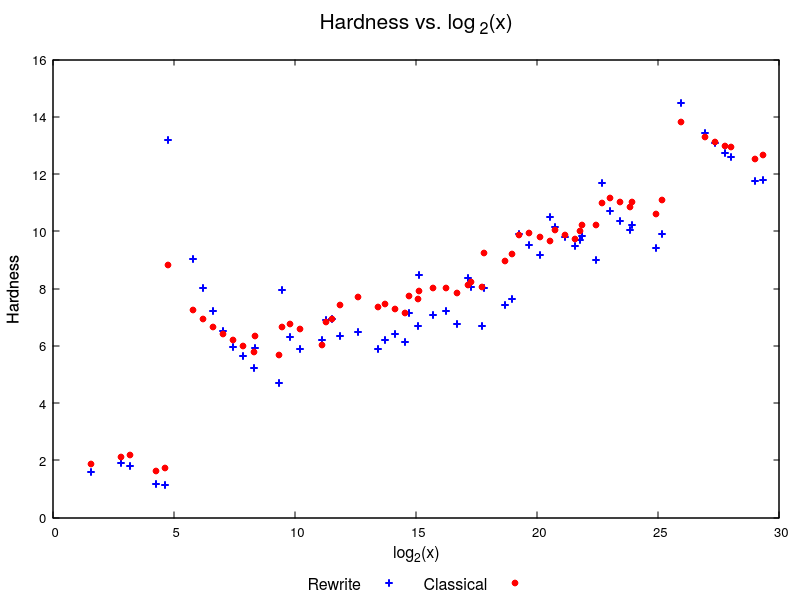
\includegraphics[scale=0.75]{ModAvoidanceAnalysisPics/RvC_vs_log.png}
    \caption{This graph compares, on the same set of input numbers, Classical Hardness as defined in chapter~\ref{sec:subhrdnspred}, and Rewrite Hardness, which is the number of steps divided by the number of input bits squared. The log of the record holding numbers, or number of bits needed, is the x-axis, and the hardness is the y-axis.}
    \label{fig:rvc_log}
\end{figure}


\section{Collatz SRS Subproblem Analysis} \label{subsec:collatzsubproblemananalysis}
Now we know that the rewrite system adds a factor of $m$ steps to attempting to prove the Collatz Conjecture, we look back at the Collatz Variants. In this section, we modify the Collatz SRS to create various ``Collatz Subproblems''. These subproblems are modifications of the SRRs for the Collatz SRS with the goal of having Collatz Subproblems that align with our previously defined Collatz Variants. We show how to create Collatz Subproblems, then run computation using our previously described program.
\subsection{Modified Base 8 Rewrite System} \label{subsec:base8rewrite}
Let us explore how we can modify the Collatz SRS to make it tie into Collatz Variants. Recall the $D$ rules of the Collatz SRS: the rules that handle the even and odd numbers:
\begin{align*}
    D_1: ad &\rightarrow d &\text{$0\Mod{2}$}\\
    D_2: bd &\rightarrow gd &\text{$1\Mod{2}$}\\
\end{align*}
Recall that $D_1$ handles $0 \Mod{2}$ (even numbers) by effectively dividing by 2, while $D_2$ handles $1 \Mod{2}$ (odd numbers)  by effectively computing $(3x+1)/2$. Also note that all input strings for these rules are just one bit, since the placeholder $d$ is not a digit. However, we can expand this input to be 3 bits and come up with 8 corresponding SRRs:
\begin{align*}
    aaad &\rightarrow aad &\text{$0\Mod{8}$}\\
    aabd &\rightarrow ebad &\text{$1\Mod{8}$}\\
    abad &\rightarrow abd &\text{$2\Mod{8}$}\\
    abbd &\rightarrow fabd &\text{$3\Mod{8}$}\\
    baad &\rightarrow bad &\text{$4\Mod{8}$}\\
    babd &\rightarrow gaad &\text{$5\Mod{8}$}\\
    bbad &\rightarrow bbd &\text{$6\Mod{8}$}\\
    bbbd &\rightarrow gbbd &\text{$7\Mod{8}$}
\end{align*}
Observe that these rules all correspond to a node in graph $G_8$: an input string strictly with symbols $a$, $b$, $c$, and $d$ corresponds to a binary number. The inputs, in order, are numbers congruent modulo to 0-7$\Mod{8}$, and the outputs are the result of dividing by 2 or multiplying by 3 and adding 1. All of the odd rules, like rule $D_2$ in the original system, are just a combination of several rules, which ensure that the output string is not longer, and it reduces a couple of steps by moving the ternary term toward the front. All of the even number node rules are just the same exact rule $D_1$ in the original system, so we can remove any even rules and replace them with the original $D_1$. We can also eliminate in odd rules any extra $a$ terms in the output that we know would be eliminated by rule $D_1$. We ended up using the following SRRs in the base 8 modification of the Collatz SRS:
\begin{align*}
    D_{8_1}: ad &\rightarrow d &\text{$0\Mod{2}$}\\
    D_{8_2}: aabd &\rightarrow ebd &\text{$1\Mod{8}$}\\
    D_{8_3}: abbd &\rightarrow fabd &\text{$3\Mod{8}$}\\
    D_{8_4}: babd &\rightarrow gd &\text{$5\Mod{8}$}\\
    D_{8_5}: bbbd &\rightarrow gbbd &\text{$7\Mod{8}$}
\end{align*}
Because these rules were constructed using only SRRs in the Collatz SRS that we know to be correct, we know these new $D$ rules, plus the $A$, $B$, and $C$ rules, are equal to the original Collatz SRS. However, they do add an extra dimension not present before. We can remove one of the rules to make it easier to prove that the derived SRS will terminate. We present a sample SRS with rule $D_{8_2}$ removed:
\begin{align*}
    D_{8_1}: ad &\rightarrow d &\text{$0\Mod{2}$}\\
    D_{8_3}: abbd &\rightarrow fbbd &\text{$3\Mod{8}$}\\
    D_{8_4}: babd &\rightarrow gd &\text{$5\Mod{8}$}\\
    D_{8_5}: bbbd &\rightarrow gbbd &\text{$7\Mod{8}$}
\end{align*}
Since we removed the SRR that corresponds to input $1 \Mod{8}$, termination of this SRS implies termination of Collatz Variant 1, as removing a rule causes any string with this input to terminate the system. This modified Collatz SRS is called Collatz Subproblem 1 in this paper. Note how removing an SRR is equivalent to adding the corresponding termination condition in Algorithm~\ref{alg:ColSP}.  We analyzed this and other Collatz Subproblems that would imply termination of unproven Collatz Variants.\par
\subsection{Defining Measures for Subproblem Analysis} \label{subsec:rewritemeasuredefs}
For the Collatz Subproblem computations, instead of defining hardness by number of odd numbers, we define hardness based off of the total steps applied, because of the fact that odd numbers add significantly more steps. Define the following numbers, given some input number $x$:
\begin{itemize}
    \item $f_r(x)$: The total number of rewrite steps in the sequence for $x$ before it converges to 1.
    \item $A$: The base avoidance set, same as used in Algorithm~\ref{alg:ColSP} and chapter~\ref{sec:subhrdnspred}. In this chapter, $A \subseteq \{1, 5, 7\}$ and $A \ne \varnothing$. 
    \item Collatz Subproblem $A$: Defined much in the same way as Collatz Variant $A$, but with SRS instead. Let $A$ be the same base avoidance set as in $\ColMod{N}{A}{b}$. For singleton sets $A$, we just write the number with no curly braces. Collatz Subprolem $A$ denotes which rewrite rule(s) are dropped from the base 8 modification of the Collatz SRS. A proof for termination of subproblem $A$ implies termination of Collatz Variant $A$.
    \item Record Sequence for Collatz Subproblem $A$: Same exact definition as in chapter~\ref{sec:subhrdnspred}. We only run rewrite systems for the record sequences we computed with the algebraic Collatz Program defined in subsection~\ref{subsec:algcomp}, as running computation for strictly the rewrite system would take an extremely long time.
    \item $R(x_i, A, b):$ The number of rewrite steps that the record sequence from Collatz Variant $\ColMod{x}{A}{b}$ takes in an SRS based off of Collatz Subproblem $A$. However, one big difference with $R$ is that we start at the sequence number $x_i$ such that index $i$ starts at the first number of the record sequence. This is necessary in order to correctly run the Collatz SRS for these various subproblems, because otherwise the Collatz SRS will terminate too early.
\end{itemize}
We define a hardness measure: $H_{SRS}$, where $H_{SRS} = \frac{R(x_i, A, b)}{\log_2^2{x}}$. This effectively computes the hardness of the SRRs that corresponds to determining termination of Collatz Variant $A$, but also takes into account the extra factor of $m$ steps that the Collatz SRS adds. The number of bits we divide by is determined by our starting number, like for the analysis of Collatz Variants.

\subsection{SRR removal analysis} \label{subsec:rewritehardness}
Figure~\ref{fig:rvslog} shows the analysis of hardness for the modified SRS with four different Collatz Subproblems: 1, 5, 7, and $\{5,7\}$. 
\begin{figure}
    \centering
    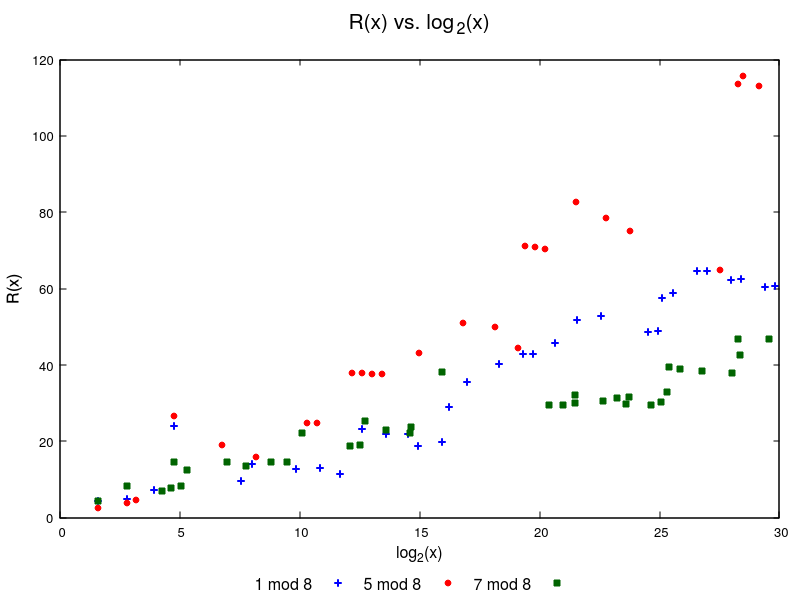
\includegraphics[scale=0.75]{ModAvoidanceAnalysisPics/R_vs_log.png}
    \caption{This graph visualizes how the $R$ values for subproblems 1, 5, and 7 compare to each other. The log of the record holding numbers, or number of bits needed, is the x-axis, and the hardness measure $R$ as defined in section~\ref{subsec:rewritemeasuredefs} is the y-axis.}
    \label{fig:rvslog}
\end{figure}
Unlike the analysis for the Collatz Variants, we have clearer separation. Subproblem 5 is the highest on almost all of its record cases. Since Collatz Variant 5 record sequences tend to grow to very large numbers, these extra bits that the large numbers generate add difficulty for the rewrite system. Further, subproblem 5 appears to get harder as the number of bits increases. Subproblem 1 exhibits the growth as numbers get bigger, but tapers off once again for numbers more than 20 bits, much like Collatz Variant 1. Subproblem 7 shows no increase as bits get larger. This suggests subproblem 7 might be easier to solve than subproblems 1 or 5. Subproblem $\{5,7\}$ has the lowest hardness, which makes sense given that it has one less rule than any of the other three subproblems.
\section{Further SRS rule modifications}\label{subsec:srsrulemod}
It is possible that the set of SRRs in the Collatz SRS can be further optimized, possibly in order to solve some of the subproblems listed in this Chapter. We present one modification of the Collatz SRS by replacing the base $D$ rules with all odd rules, and look at the results of doing so.
\subsection{Removing even rule from the Collatz SRS}\label{subsubsec:evenruleremove}
It is possible to replace both $D_1$ and $D_2$ in the Collatz SRS with the following set of rules that calculates with strictly odd numbers:
\begin{align*}
    D_{o1}: bbd &\rightarrow gbd &\text{$3\Mod{4}$}\\
    D_{o2}: aabd &\rightarrow ebd &\text{$1\Mod{8}$}\\
    D_{o3}: babd &\rightarrow bd &\text{$5\Mod{8}$}
\end{align*}
Notice that rule $D_{o1}$ and $D_{o2}$ are borrowed from the base 8 modification of the Collatz SRS. $D_{o1}$ combines both rule $D_{8_3}$ and $D_{8_5}$, removing the leading $a$ or $b$, respectively, and letting the $A$, $B$, and $C$ rules determine the next symbol(s). Rule $D_{o2}$ is the same as rule $D_{8_2}$.\par
Rule $D_{o3}$ is not as intuitive at first glance, but we can look at rule $D_{8_4}$, which has the same input as $D_{o3}$, and see that the output is the same as the normal $D_2$ rule, so we can ``step backwards'' using rule $D_2$ to allow for us to get $bd$ as our output, and hence, have a full set of correct $D$ rules that go from odd number to odd number.\par
Observe that all of the $D_o$ rules have a left handed side and a right handed side ending with $bd$. As a consequence, we can remove the $b$ symbol in the second to last symbol for both the input string and the rules, resulting in the following SRRs:
\begin{align*}
    D_{o1^*}: bd &\rightarrow gd &\text{$3\Mod{4}$}\\
    D_{o2^*}: aad &\rightarrow ed &\text{$1\Mod{8}$}\\
    D_{o3^*}: bad &\rightarrow d &\text{$5\Mod{8}$}
\end{align*}
\subsection{Change in Rewrite Steps}
\begin{figure}
    \centering
    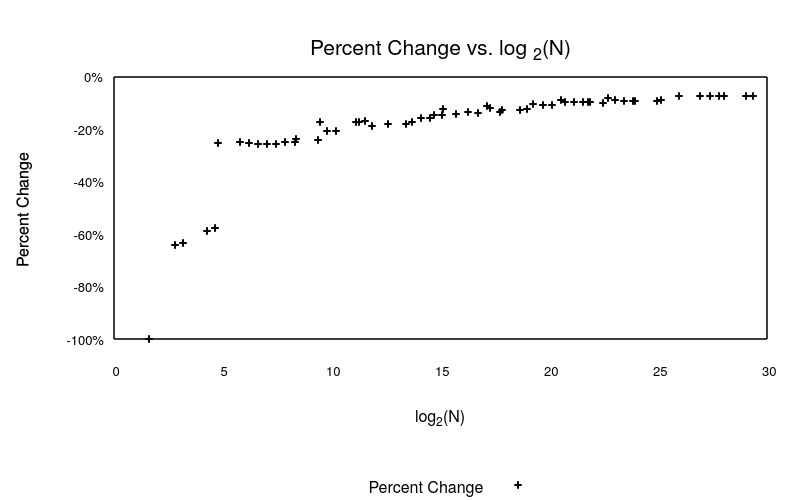
\includegraphics[scale=0.75]{ModAvoidanceAnalysisPics/Percent_Change.png}
    \caption{This graph shows what percentage the odd rules change the rewrite steps, as opposed to the original Collatz SRS. The log of the record holding numbers, or number of bits needed, is the x-axis, and the percent decrease is the y-axis.}
    \label{fig:percent_decrease}
\end{figure}
Figure~\ref{fig:percent_decrease} shows the percentage change for Classical Hardness records when the $D_o$ rules are used compared to the normal $D$ rules. Lower numbers tend to have a larger percentage of decrease, but as the numbers get larger, the decrease percentage reduces by quite a bit. This is probably because records for larger numbers tend to have more odd numbers, meaning many more rewrite steps than lower numbers. That said, this modification to the rewrite system does overall reduce the number of rewrite steps. Other SRR modifications for the Collatz SRS should be considered, as the right set of clever rules may prove termination of Collatz Subproblems, and perhaps, even prove that the Collatz Conjecture terminates.
